\section{Sigma协议:范例}

到目前为止,我们所见过的唯一的 Sigma 协议是 Schnorr 协议,它允许一个证明者说服一个持怀疑态度的验证者,它``知道"一个给定群元素的离散对数,却不向验证者透露任何关于离散对数的信息。在本节中,我们将介绍另外几个 Sigma 协议的例子。这些例子不仅有助于充实 Sigma 协议的普遍理论,也有许多实际应用,其中的一些我们将在下面讨论。

\subsection{用于表示的 Okamoto 协议}\label{subsec:19-5-1}

令 $\mathbb{G}$ 是一个由 $g\in\mathbb{G}$ 生成的素阶 $q$ 的循环群,$h\in\mathbb{G}$ 是任意群元素。我们现在将 $h$ 看作是一个系统参数。所谓系统参数会在系统初始化时一次性生成,并对所有参与方公开。对于一个 $u\in\mathbb{G}$,如果给定 $g$ 和 $h$,可以使用一个数对 $(\alpha,\beta)\in\mathbb{Z}_q^2$ 来表示 $u$,方法是 $g^\alpha h^\beta=u$。

Okamoto 协议允许证明者说服持怀疑态度的验证者,它``知道"一个给定的 $u\in\mathbb{G}$ 的表示,但不需要向验证者透露任何有关该表示的具体信息。更确切地说,它是一个对于关系:
\begin{equation}\label{eq:19-11}
	\mathcal{R}=\bigg\lbrace
	\big((\alpha,\beta),u\big)\in\mathbb{Z}_q^2\times\mathbb{G}:g^\alpha h^\beta=u
	\bigg\rbrace
\end{equation}
的 Sigma 协议。陈述 $u\in\mathbb{G}$ 的一个见证 $u$ 是一个使得 $g^\alpha h^\beta=u$ 成立的数对 $(\alpha,\beta)\in\mathbb{Z}_q^2$,即 $u$ 的一个表示。因此,在这个例子中,每个陈述都对应着多个见证,准确的说是 $q$ 个见证。

通常假定 Okamoto 协议的挑战空间 $\mathcal{C}$ 是 $\mathbb{Z}_q$ 的一个子集。协议 $(P,V)$ 按如下方式运行,其中证明者 $P$ 由 $((\alpha,\beta),u)\in\mathcal{R}$ 初始化,验证者 $V$ 由 $u\in\mathbb{G}$ 初始化:
\begin{enumerate}
	\item $P$ 计算:
	$$
    \alpha_{\rm t}\overset{\rm R}\leftarrow\mathbb{Z}_q,~~
    \beta_{\rm t}\overset{\rm R}\leftarrow\mathbb{Z}_q,~~
    u_{\rm t}\leftarrow g^{\alpha_{\rm t}}h^{\beta_{\rm t}}
    $$
    并将承诺 $u_{\rm t}$ 发送给 $V$;
	\item $V$ 选取$c\overset{R}\leftarrow\mathcal{C}$,然后将挑战 $c$ 发送给 $P$;
	\item $P$ 计算:
	$$
    \alpha_{\rm z}\leftarrow\alpha_{\rm t}+\alpha c\in\mathbb{Z}_q,~~
    \beta_{\rm z}\leftarrow\beta_{\rm t}+\beta c\in\mathbb{Z}_q
    $$
    并将应答 $(\alpha_{\rm z}, \beta_{\rm z})$ 发送给 $V$;
	\item $V$ 检查$g^{\alpha_{\rm z}}h^{\beta_{\rm z}}\overset{?}=u_{\rm t}\cdot u^c$是否成立。如果是,$V$ 输出 $\mathsf{accept}$,否则 $V$ 输出 $\mathsf{reject}$。
\end{enumerate}
参见图 \ref{fig:19-6}。

\begin{figure}
  \centering
  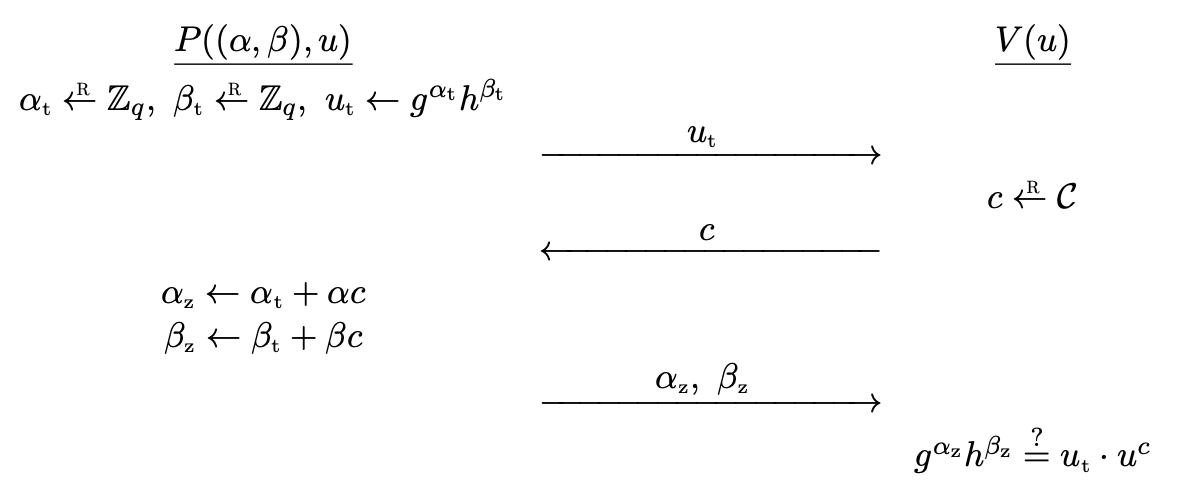
\includegraphics[width=0.75\linewidth]{figures/chapter19/fig6.png}
  \caption{Okamoto 协议}
  \label{fig:19-6}
\end{figure}

\begin{theorem}
Okamoto 协议是针对式 \ref{eq:19-11} 中定义的关系$\mathcal{R}$的一个 Sigma 协议。此外,Okamoto 协议提供知识健全性,且是特殊 HVZK 的。
\end{theorem}

\begin{proof}
显然,Okamoto 协议具有 Sigma 协议所要求的语法结构。陈述 $u\in\mathbb{G}$ 的一个接受对话形如:
$$
(u_{\rm t},c,(\alpha_{\rm z},\beta_{\rm z})) \text{~~s.t.~~} g^{\alpha_{\rm z}}h^{\beta_{\rm z}}=u_{\rm t}\cdot u^c
$$

\noindent
\emph{正确性.}
我们首先必须验证 Okamoto 协议是否满足基本的正确性要求,即诚实证明者和诚实验证者之间的交互总是能够产生一个接受对话。这很容易验证,因为如果:
$$
u_{\rm t}=g^{\alpha_{\rm t}}h^{\beta_{\rm t}},~~
\alpha_{\rm z}=\alpha_{\rm t}+\alpha c,~~
\beta_{\rm z}=\beta_{\rm t}+\beta c
$$
则我们有:
$$
g^{\alpha_{\rm z}}h^{\beta_{\rm z}}=
g^{\alpha_{\rm t}+\alpha c}h^{\beta_{\rm t}+\beta c}=
g^{\alpha_{\rm t}}h^{\beta_{\rm t}}\cdot(g^\alpha h^\beta)^c=
u_{\rm t}\cdot u^c
$$

\noindent
\emph{知识健全性.}
我们下面证明 Okamoto 协议提供知识健全性。假设我们现在有两个陈述 $u$ 的接受对话:
$$
(u_{\rm t},c,(\alpha_{\rm z},\beta_{\rm z})),~~
(u_{\rm t},c',(\alpha_{\rm z}',\beta_{\rm z}'))
$$
其中 $c\neq c'$。我们需要说明如何从这两个对话中有效提取 $u$ 的表示。这里的计算与 Schnorr 协议中的计算非常类似。注意到:
$$
g^{\alpha_{\rm z}}h^{\beta_{\rm z}}=u_{\rm t}\cdot u^c,~~
g^{\alpha_{\rm z}'}h^{\beta_{\rm z}'}=u_{\rm t}\cdot u^{c'}
$$
将第一个等式除以第二个等式,$u_{\rm t}$ 就被抵消了,于是我们有:
$$
g^{\Delta\alpha}h^{\Delta\beta}=u^{\Delta c},~~~~
\Delta\alpha:=\alpha_{\rm z}-\alpha_{\rm z}',~~
\Delta\beta:=\beta_{\rm z}-\beta_{\rm z}',~~
\Delta c:=c-c'
$$
因此,见证提取器可以用:
$$
\alpha\leftarrow{\Delta\alpha}/{c},~~
\beta\leftarrow{\Delta\beta}/{c}
$$
有效地计算出 $u$ 的一个表示 $(\alpha,\beta)\in\mathbb{Z}_q^2$。需要注意的是,由于 $c\neq c'$,$\Delta c$ 在 $\mathbb{Z}_q$ 中是可逆的。我们在这里利用了$q$是一个素数这个事实。

\vspace{5pt}

\noindent
\emph{特殊 HVZK.}
最后,我们通过给出一个模拟器来证明 Okamoto 协议是特殊 HVZK 的。这同样与 Schnorr 协议非常相似。对于输入 $u\in\mathbb{G}$ 和 $c\in\mathcal{C}$,模拟器计算:
$$
\alpha_{\rm z}\overset{\rm R}\leftarrow\mathbb{Z}_q,~~
\beta_{\rm z}\overset{\rm R}\leftarrow\mathbb{Z}_q,~~
u_{\rm t}\leftarrow{g^{\alpha_{\rm z}}h^{\beta_{\rm z}}}/{u^c}
$$
并输出 $(u_{\rm t},(\alpha_{\rm z},\beta_{\rm z}))$。可以发现,输出总是会产生一个符合要求的接受对话。

下面我们论证,当 $c\in\mathcal{C}$ 是随机选出的时候,模拟器在输入 $u,c$ 上的输出具有正确的分布。注意到在真实的对话中,$c$,$\alpha_{\rm z}$ 与 $\beta_{\rm z}$ 相互独立,其中 $c$ 在 $\mathcal{C}$ 上均匀分布,$\alpha_{\rm z}$ 和 $\beta_{\rm z}$ 在 $\mathbb{Z}_q$ 上均匀分布。此外,如果给定 $c$、$\alpha_{\rm z}$ 和 $\beta_{\rm z}$,$u_{\rm t}$ 的值由方程:

$$
g^{\alpha_{\rm z}}h^{\beta_{\rm z}}=u_{\rm t}\cdot u^c
$$
唯一决定。而这显然与模拟器的输出分布是一致的。
\end{proof}

\subsection{用于 DH 三元组的 Chaum-Pedersen 协议}\label{subsec:19-5-2}

Chaum-Pedersen 协议允许证明者在不向验证者透露任何其他信息的情况下,说服一个持怀疑态度的验证者相信一个给定的三元组是DH 三元组。

令 $\mathbb{G}$ 是一个 $q$ 阶循环群,其中 $q$ 是素数,$g\in\mathbb{G}$ 是生成元。回忆一下 10.5 节,对于 $\alpha,\beta,\gamma\in\mathbb{Z}_q$,如果 $\gamma=\alpha\beta$,我们就称元组 $(g^\alpha,g^\beta,g^\gamma)$ 为一个 DH 三元组 (DH-triple)。等价地,当且仅当存在 $\beta\in\mathbb{Z}_q$ 使得 $v=g^\beta$且$w=u^\beta$ 时,元组 $(u,v,w)$ 才是一个 DH 三元组。

Chaum-Pedersen 协议是关系:
\begin{equation}\label{eq:19-12}
\mathcal{R}:=\bigg\lbrace
\big(\beta, (u,v,w)\big)\in\mathbb{Z}_q\times\mathbb{G}^3:v=g^\beta, w=u^\beta
\bigg\rbrace
\end{equation}
上的 Sigma 协议。陈述 $(u,v,w)\in\mathbb{G}^3$ 的见证是使得 $v=g^\beta$ 且 $w=u^\beta$ 的一个 $\beta\in\mathbb{Z}_q$。因此,当且仅当陈述是一个 DH 三元组时,它才会存在一个见证。 与我们之前介绍的其它例子不同,在 Chaum-Pedersen 协议中,并非所有的陈述都必然存在见证。 

图 \ref{fig:19-7} 是 Chaum-Pedersen 协议 $(P,V)$ 的流程图,挑战空间 $\mathcal{C}$ 是 $\mathbb{Z}_q$ 的一个子集。

\begin{figure}
  \centering
  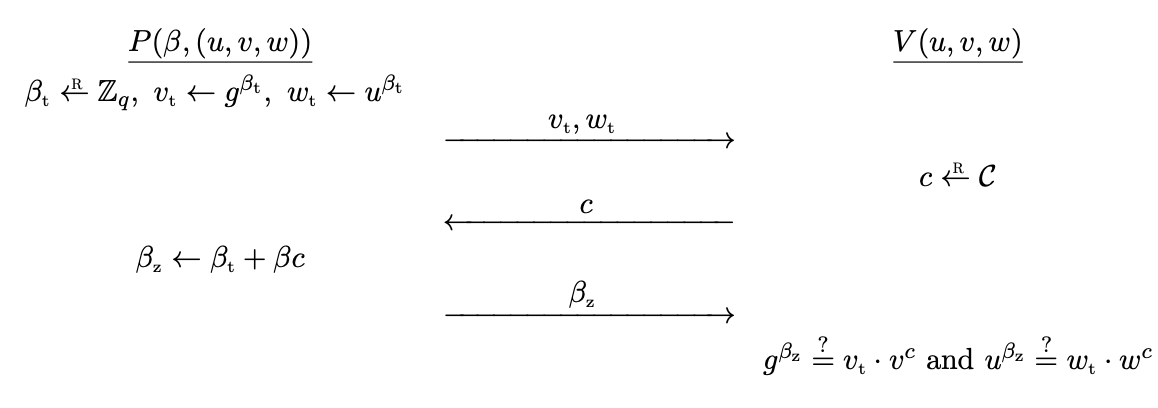
\includegraphics[width=0.75\linewidth]{figures/chapter19/fig7.png}
  \caption{Chaum-Pedersen 协议}
  \label{fig:19-7}
\end{figure}

\begin{theorem}
Chaum-Pedersen 协议是式 \ref{eq:19-12} 中定义的关系$\mathcal R$上的一个 Sigma 协议。此外,Chaum-Pedersen 协议提供知识健全性,且是特殊 HVZK 的。
\end{theorem}

\begin{proof}
显然,Chaum-Pedersen 协议具有 Sigma 协议所要求的语法结构。陈述 $(u,v,w)\in\mathbb{G}^3$ 的一个接受对话形如:
$$
((v_{\rm t},w_{\rm t}),c,\beta_{\rm z}) \text{~~s.t.~~} 
g^{\beta_{\rm z}}=v_{\rm t}\cdot v^c,~~
y^{\beta_{\rm z}}=w_{\rm t}\cdot w^c
$$
不难证明,一个诚实证明者与一个诚实验证者之间总是能够产生接受对话。

\noindent
\emph{知识健全性.}
假设我们有两个陈述 $(u,v,w)$ 的接受对话
$$
((v_{\rm t},w_{\rm t}),c,\beta_{\rm z}),~~
((v_{\rm t},w_{\rm t}),c',\beta_{\rm z}')
$$
其中 $c\neq c'$。不难发现
$$
\beta:={\Delta\beta}/{\Delta c}
$$
是陈述 $(u,v,w)\in\mathbb{G}^3$ 对应的见证,其中$\Delta\beta:=\beta_{\rm z}-\beta_{\rm z}'$,$\Delta c:=c-c'$。

\vspace{5pt}

\noindent
\emph{特殊 HVZK.}
对于输入 $(u,v,w)\in\mathbb{G}^3$ 和 $c\in\mathcal{C}$ 时,模拟器计算:
$$
\beta_{\rm z}\overset{\rm R}\leftarrow\mathbb{Z}_q,~~
v_{\rm t}\leftarrow{g^{\beta_{\rm z}}}/{v^c},~~
w_{\rm t}\leftarrow{u^{\beta_{\rm z}}}/{w^c}
$$
并输出 $((v_{\rm t},w_{\rm t}),c,\beta_{\rm z})$。可以发现,输出总是会产生一个符合要求的接受对话。

下面我们论证,当 $c\in\mathcal{C}$ 是随机选出的时候,模拟器在输入 $((u,v,w),c)$ 上的输出具有正确的分布。注意到在真实的对话中,$c$ 和 $\beta_{\rm z}$ 相互独立,其中 $c$ 在 $\mathcal{C}$ 上均匀分布,$\beta_{\rm z}$ 在 $\mathbb{Z}_q$ 上均匀分布。此外,如果给定 $c$ 和 $\beta_{\rm z}$,$v_{\rm t}$ 和 $w_{\rm t}$ 的值由
$$
g^{\beta_{\rm z}}=v_{\rm t}\cdot v^c, ~~
u^{\beta_{\rm z}} =w_{\rm t}\cdot w^c
$$
唯一决定。而这显然与模拟器的输出分布是一致的。
\end{proof}

\subsection{用于任意线性关系的 Sigma 协议}\label{subsec:19-5-3}

读者可能已经注意到 Schnorr、Okamoto 和 Chaum-Pedersen 协议之间的某些相似之处。事实上,它们都是用于证明一组元素之间线性关系的通用 Sigma 协议的特例。

与之前一样,令 $\mathbb{G}$ 是一个 $q$ 阶循环群,其中 $q$ 是素数,$g\in\mathbb{G}$ 是生成元。考察形如:
\begin{equation}\label{eq:19-13}
\phi(x_1,\dots,x_n):=
\left\{
~u_1=\prod^n_{j=1}g_{1j}^{x_j} ~~\land~~\cdots~~\land~~ u_m=\prod^n_{j=1}g_{mj}^{x_j}~
\right\}
\end{equation}
的布尔表达式 $\phi$。其中所有的 $g_{ij}$ 和 $u_i$ 都是 $\mathbb{G}$ 中的元素,这些元素中的有些可以是系统参数甚至是常数,有些是表达式特有的。$\phi$ 中的 $x_i$ 是公式的变量。当我们给 $x_1,\dots,x_n$ 赋 $\mathbb{Z}_q$ 中的值时,如果式 \ref{eq:19-13} 中的所有等式都成立,$\phi$ 就会输出 true。

对于这类公式的集合 $\mathcal{F}$,我们可以定义关系:
\begin{equation}\label{eq:19-14}
\mathcal{R}:=
\bigg\lbrace
\Big(
(\alpha_1,\dots,\alpha_n),\phi
\Big)
\in\mathbb{Z}_q^n\times\mathcal{F}: ~\phi(x_1,\dots,x_n)={\rm{true}}~
\bigg\rbrace
\end{equation}
因此,陈述是一个表达式 $\phi\in\mathcal{F}$,$\phi$ 的见证是能使得表达式 $\phi$ 输出 true 的 $x_1,\dots,x_n$ 的一组赋值 $(\alpha_1,\dots,\alpha_n)\in\mathbb{Z}_q^n$。我们之所以称其为``线性"关系集,是因为如果我们取离散对数,式 \ref{eq:19-13} 就可以改写为如下的线性方程组:
$$
{\rm\mathsf{Dlog}}_g(u_j)=\sum_{j=1}^nx_i\cdot {\rm\mathsf{Dlog}}_g(g_{ij})~~~~(i=1,2,\dots,m)
$$
而见证就是上述线性方程组的一组解。

\begin{figure}
  \centering
  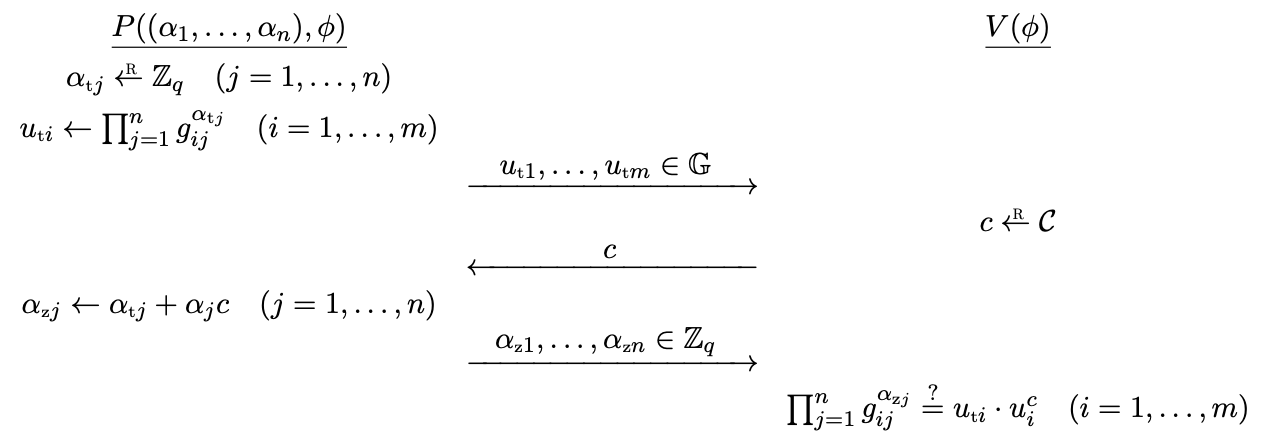
\includegraphics[width=0.85\linewidth]{figures/chapter19/fig8.png}
  \caption{通用线性协议}
  \label{fig:19-8}
\end{figure}

图 \ref{fig:19-8} 展示了关系 $\mathcal{R}$ 上的\textbf{通用线性协议 (generic linear protocol)} $(P,V)$。证明者拥有 $\phi$ 和见证 $(\alpha_1,\dots,\alpha_n)\in\mathbb{Z}_q^n$,挑战空间 $\mathcal{C}$ 是 $\mathbb{Z}_q$ 的一个子集。这样,到目前为止我们所介绍的所有 Sigma 协议都是这个通用线性协议的特例:
\begin{itemize}
	\item Schnorr 协议对应着 $\phi_1(x):=\{u=g^x\}$ 的情况。
	\item Okamoto 协议对应着 $\phi_2(x,y):=\{u=g^xh^y\}$ 的情况。
	\item Chaum-Pedersen 协议对应着 $\phi_3(x):=\{v=g^x\land w=u^x\}$ 的情况。
\end{itemize}

我们可以通过模仿Schnorr、Okamoto和Chaum-Pedersen的相应定理的证明来证明以下定理。我们把它作为一个练习留给读者。

\begin{theorem}\label{theo:19-11}
图 \ref{fig:19-8} 所描述的通用线性协议是式 \ref{eq:19-14} 中定义的关系 $\mathcal R$ 上的一个 Sigma 协议。此外,该协议提供知识健全性,且是特殊 HVZK 的。
\end{theorem}

我们还可以进一步泛化这个通用线性协议,方法是允许式 \ref{eq:19-13} 中的各个方程定义在不同的群上。唯一的要求是所有群都有相同的素阶 $q$。这种更通用的线性协议的典型出现场景是有两类方程,其中一类定义在密码学所感兴趣的群 $\mathbb{G}$ 上,群的阶为素数 $q$;另一类定义在 $\mathbb{Z}_q$ 上,其形式为 $\kappa_i=\sum_{j=1}^n\lambda_{ij}x_j$,其中 $\kappa_i$ 和 $\lambda_{ij}$ 是 $\mathbb{Z}_q$ 中的元素。

\subsection{一种用于同态原像的 Sigma 协议}

到目前为止我们介绍的所有 Sigma 协议,包括通用线性协议,都可以用群同态的语言来更清楚、更简洁地描述。令 $\mathbb{H}_1$ 和 $\mathbb{H}_2$ 是两个阶已知的有限阿贝尔群,$\psi:\mathbb{H}_1\to\mathbb{H}_2$ 是一个群同态。我们将群 $\mathbb{H}_1$ 中的运算表示为加法形式,将群 $\mathbb{H}_2$ 中的运算表示为乘法形式。

\begin{figure}
  \centering
  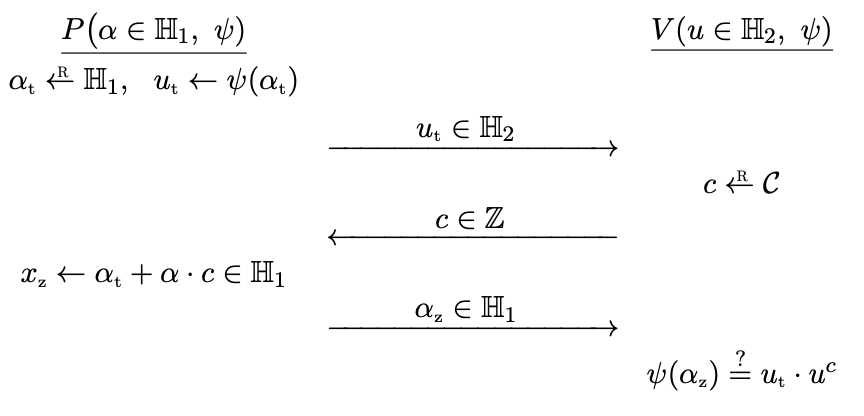
\includegraphics[width=0.6\linewidth]{figures/chapter19/fig9.png}
  \caption{用于同态原像的 Sigma 协议}
  \label{fig:19-9}
\end{figure}

令 $u\in\mathbb{H}_2$。图 \ref{fig:19-9} 展示了一个 Sigma 协议,它允许证明者说服验证者它``知道" $u$ 在 $\psi$ 下的原像。具体地,该协议是关系:
\begin{equation}\label{eq:19-15}
\mathcal{R}:=\bigg\lbrace
\Big(\alpha,(u,\psi)\Big)\in\mathbb{H}_1\times(\mathbb{H}_1\times\mathcal{F}):\psi(\alpha)=u
\bigg\rbrace
\end{equation}
上的一个 Sigma 协议。其中 $\alpha\in\mathbb{H}_1$ 是 $u\in\mathbb{H}_2$ 在 $\psi$ 下的原像。图 \ref{fig:19-9} 中的证明者持有见证 $\alpha\in\mathbb{H}_1$,验证者持有像 $u\in\mathbb{H}_2$,双方共有 $(\mathbb{H}_1,\mathbb{H}_2,\psi)$。挑战空间 $\mathcal{C}$ 为 $\{0,1,\dots,N-1\}\subseteq\mathbb{Z}$,其中 $N$ 为特定整数。

下面让我们看看这个协议是如何包含到目前为止所有的 Sigma 协议实例的。令 $\mathbb{G}$ 是一个素阶 $q$ 的群,且有生成元 $g,h,u\in\mathbb{G}$:
\begin{itemize}
	\item Okamoto 协议对应着 $\mathbb{H}_1:=\mathbb{Z}_q^2$,$\mathbb{H}_2:=\mathbb{G}$ 且 $\psi_1(x,y):=g^xh^y$ 的特殊情况。
	\item Chaum-Pedersen 协议对应着
	$$\mathbb{H}_1:=\mathbb{Z}_q,~~\mathbb{H}_2:=\mathbb{G}^2, ~~\psi_2(x):=(g^x,u^x)$$
	的特殊情况。我们甚至可以令 $\mathbb{H}_2=\mathbb{G}_1\times\mathbb{G}_2$,其中 $g\in\mathbb{G}_1$,$u\in\mathbb{G}_2$,并且 $|\mathbb{G}_1|=|\mathbb{G}_2|$。那么对于一个给定的 $(v,w)\in\mathbb{G}_1\times\mathbb{G}_2$,提供$(v, w)$ 在 $\psi_2$ 上的一个原像与计算群 $\mathbb{G}_1$ 和 $\mathbb{G}_2$ 上的离散对数问题 $\mathsf{Dlog}_g(v)=\mathsf{Dlog}_u(w)$ 等价。
	\item 图 \ref{fig:19-8} 中的通用线性协议对应着
	$$
    \mathbb{H}_1:=(\mathbb{Z}_q)^n,~~
    \mathbb{H}_2:=\mathbb{G}^m,~~
    \psi_3(x_1,\dots,x_n):=
    \left(
    ~\prod_{j=1}^ng_{1j}^{x_j},~\dots,~\prod_{j=1}^ng_{mj}^{x_j}~
    \right)
    $$
    的特殊情况。其中,对于所有的$i=1,\dots,m$和$j=1,\dots,n$,都有$g_{ij}\in\mathbb{G}$。
\end{itemize}
我们可以很容易地验证 $\psi_1,\psi_2,\psi_3$ 的映射都是群同态的。通过在图 \ref{fig:19-9} 中的协议使用这些同态映射,我们可以得到本节中介绍的所有 Sigma 协议实例。

\begin{theorem}\label{theo:19-12}
图 \ref{fig:19-9} 中的协议是式 \ref{eq:19-15} 中定义的关系 $\mathcal R$ 上的一个 Sigma 协议。此外,该协议是特殊 HVZK 的,而且只要 $|\mathbb{H}_1|\times|\mathbb{H}_2|$ 的最小素因子至少是 $|\mathcal{C}|$,该协议就提供知识健全性。
\end{theorem}

定理 \ref{theo:19-12} 的证明完全模仿了 Schnorr 协议相应定理的证明。对 $|\mathbb{H}_1|\times|\mathbb{H}_2|$ 的最小素因子的下限要求,是为了确保见证提取器可以从两个接受对话 $(u_{\rm t},c,\alpha_{\rm z})$ 和 $(u_{\rm t},c',\alpha_{\rm z}')$ 中获得一个映射 $\psi$ 的原像。就如同在 Schnorr 协议中的见证提取器中那样,我们可以得到$\psi(\Delta\alpha)=u^{\Delta c}$,其中$\Delta\alpha:=(\alpha_z-\alpha_z')\in\mathbb{H}_1$,$\Delta c=(c-c')\in\mathbb{Z}$。限制 $|\mathbb{H}_1|$ 和 $|\mathbb{H}_2|$ 素因子的下界是为了确保(1)我们可以在 $\mathbb{H}_1$ 中用 $\Delta c$ 除以 $\Delta\alpha$,并且(2)我们可以在等式两边同时升幂 $((\Delta c)^{-1}\mod |\mathbb{H}_2|)\in\mathbb{Z}$,以求得等式右项的 $\Delta c$ 次方根。然后,我们就可以得到$\psi({\Delta\alpha}/{\Delta c})=u$,因此 ${\Delta\alpha}/{\Delta c}\in\mathbb{H}_1$ 就是 $u\in\mathbb{H}_2$ 在映射 $\psi$ 下的原像。

\subsection{一种用于 RSA 的 Sigma 协议}\label{subsec:19-5-5}

为了避免读者认为 Sigma 协议只适用于与离散对数有关的问题,我们下面介绍一个与 RSA 有关的协议。

令 $(n,e)$ 是一个 RSA 公钥,$e$ 是一个素数。我们将 $(n,e)$ 视为一个系统参数。Guillou-Quisquater (GQ) 协议允许证明者说服持怀疑态度的验证者,它``知道" $y\in\mathbb{Z}_n^*$ 的一个 $e$ 次方根,而不透露任何其他信息。更确切地说,GQ 协议是关系:
\begin{equation}\label{eq:19-16}
\mathcal{R}=
\bigg\lbrace
(x,y)\in\mathbb{Z}_n^*\times\mathbb{Z}_n^*:x^e=y
\bigg\rbrace
\end{equation}
上的一个 Sigma 协议。陈述 $y\in\mathbb{Z}_n^*$ 的见证是 $x\in\mathbb{Z}_n^*$,满足 $x^e=y$。由于 $(n,e)$ 是一个 RSA 公钥,因此由 $x\in\mathbb{Z}_n^*$ 到 $y=x^e\in\mathbb{Z}_n^*$ 的映射是一个双射。因此每个陈述都对应着唯一的见证。

\begin{figure}
  \centering
  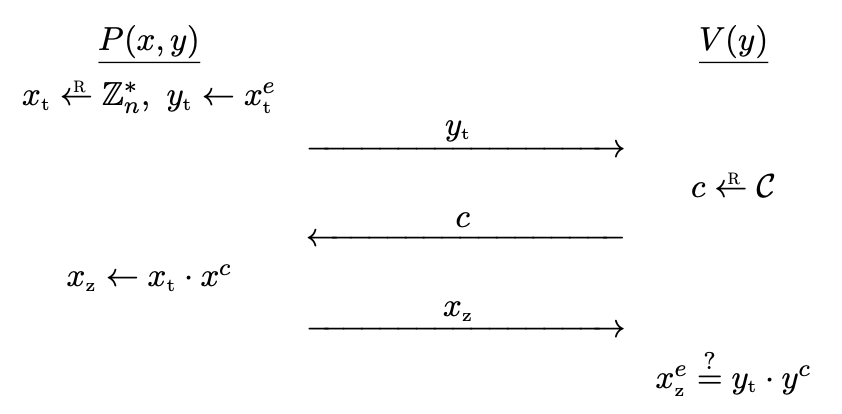
\includegraphics[width=0.6\linewidth]{figures/chapter19/fig10.png}
  \caption{Guillou-Quisquater 协议}
  \label{fig:19-10}
\end{figure}


图 \ref{fig:19-10} 展示了 GQ 协议 $(P,V)$ 的工作流程。其挑战空间 $\mathcal{C}$ 是 $\{0,\dots,e-1\}$ 的一个子集。需要注意的是,当 $e$ 很小时,挑战空间也很小。如果需要,我们可以用练习 19.5 中介绍的方法将其扩大。然而在使用该协议时,我们通常会将 $e$ 设定为一个大素数来确保挑战空间是足够大的。

图 \ref{fig:19-10} 中的 GQ 协议也是图 \ref{fig:19-9} 中展示的用于同态原像的 Sigma 协议的一个特例。此时群同态是 $\psi:\mathbb{Z}_n^*\to\mathbb{Z}_n^*$,定义为 $\psi(x)=x^e$。然而,我们无法像定理 \ref{theo:19-12} 那样证明 GO 协议提供知识健全性,因为群 $\mathbb{Z}_n^*$ 的阶是未知的。相反地,我们必须对这些属性进行单独证明。我们有下面的定理。

\begin{theorem}
GQ协议是式 \ref{eq:19-16} 中定义的关系$\mathcal R$上的一个Sigma协议。此外,它提供知识健全性,并且是特殊HVZK的。
\end{theorem}

\begin{proof}
$y$ 的一个接受对话形如 $(x_{\rm t},c,x_{\rm z})$,其中 $x^e_{\rm z}=y_{\rm t}\cdot y^c$。读者很容易验证基本的正确性要求,即一个诚实证明者和一个诚实验证者之间的交互总是会产生一个接受对话。

\vspace{5pt}

\noindent
\emph{知识健全性.}
下面我们将证明 GQ 协议具备知识健全性。假设我们有两个陈述 $y$ 的接受对话 $(x_{\rm t},c,x_{\rm z})$ 和 $(x_{\rm t},c',x_{\rm z}')$,其中 $c\neq c'$。我们必须证明能够有效计算出 $y$ 的 $e$ 次方根。观察到:
$$
x^e_{\rm z}=y_{\rm t}\cdot y^c,~~
(x_{\rm z}')^e=y_{\rm t}\cdot y^{c'}
$$
将第一个方程除以第二个方程,可以得到:
$$
(\Delta x)^e=y^{\Delta c}
$$
其中:$\Delta x:={x_{\rm z}}/{x_{\rm z}'}$,$\Delta c:=c-c'$。由于 $c\neq c'$,且 $c$ 和 $c'$ 都属于区间 $\{0,\dots,e-1\}$,因此有 $0<|\Delta c|<e$,所以 $e\nmid\Delta c$。此外由于 $e$ 是素数,所以 $\gcd(e,\Delta c)=1$。因此当给定 $e$,$f:=\Delta c$,$w:=\Delta x$ 时,我们可以利用定理 10.6 求得 $y$ 的 $e$ 次方根。

读者应该注意到,这里给出的从两个接受对话中计算 RSA 逆变换的技术与定理 10.7 的证明中使用的方法基本相同。事实上,这两个接受对话制造了哈希函数 $H_{\rm rsa}(a,b)=a^ey^b$ 上的一次碰撞 $((x_{\rm z},-c\mod e),(x_{\rm z}',-c'\mod e))$。

\vspace{5pt}

\noindent
\emph{特殊 HVZK.}
最后,我们通过给出一个模拟器来证明 GQ 协议是特殊 HVZK 的。对于输入 $y\in\mathbb{Z}_n^*$ 和 $c\in\mathcal{C}$,模拟器计算:
$$
x_{\rm z}\overset{\rm R}\leftarrow\mathbb{Z}_n^*,~~
y_{\rm t}\leftarrow{x_{\rm z}^e}/{y^c}
$$
并输出 $(y_{\rm t},x_{\rm z})$。注意到在真实的对话中,$c$ 和 $x_{\rm z}$ 是相互独立的,$c$ 在 $\mathcal{C}$ 上均匀分布,$x_z$ 在 $\mathbb{Z}_n^*$ 上均匀分布。此外,如果给定 $c$ 和 $x_z$,$y_t$ 的值由方程$x^e_{\rm z}=y_{\rm t}\cdot y^c$唯一决定。而这显然与模拟器的输出分布是一致的。
\end{proof}